% =====================================================================
% WORKSHOP VERSION -- 8 content pages, NeurIPS 2026 workshop format.
%
% Target venues: NewInML (2-8pp), CL4FMAgents regular track (8pp).
% For the 4-page venues (AXIOM, EvoRobust) cut Section 5 to one
% paragraph and move Section 2 wholly to the appendix; see
% docs/WORKSHOP_SUBMISSION_GUIDE.md.
%
% STRUCTURE follows the convention in this literature rather than the
% full-paper shape: related work lives in the appendix (as in
% Gerstgrasser et al.), results are reported with the experiment that
% produced them, and limitations sit inside the discussion instead of
% carrying their own section.
%
% EVERY RESULT NUMBER is a macro from tables/pilot_macros.tex, generated
% by scripts/generate_pilot_outputs.py from the chain artifacts. This
% file and paper/main.tex therefore cannot disagree about a number.
% =====================================================================

% The venue style file. Drop neurips_2026.sty beside this file and it is
% used automatically; without it we fall back to a geometry that matches
% the NeurIPS text block (5.5in x 9in), so local page counts are honest.
\documentclass{article}
\IfFileExists{neurips_2026.sty}{%
  \usepackage[final]{neurips_2026}%
}{%
  \usepackage[letterpaper,textwidth=5.5in,textheight=9in,centering]{geometry}%
  \PackageWarningNoLine{workshop}{neurips_2026.sty not found -- using a text
    block of the same dimensions. Page count is representative; add the real
    style file before submitting}%
}

\usepackage{amsmath,amssymb,booktabs,graphicx,hyperref}
\graphicspath{{../results/figures/}{./}}
\usepackage{tikz}
\usetikzlibrary{arrows.meta,positioning}

% AUTO-GENERATED by scripts/generate_pilot_outputs.py. DO NOT EDIT VALUES BY HAND.
% Every result number quoted in paper/sections/ is defined here and computed
% from chain_result.json artifacts, so prose cannot drift from the run.
% run: primary_pilot_2026-08-18
\newcommand{\PilotCVHigh}{1.08}
\newcommand{\PilotCVLow}{0.41}
\newcommand{\PilotCeiling}{750{,}000}
\newcommand{\PilotChains}{25}
\newcommand{\PilotHorizon}{10}
\newcommand{\PilotJointSelHigh}{0.019}
\newcommand{\PilotJointSelLow}{-0.003}
\newcommand{\PilotJointSelPct}{0.36}
\newcommand{\PilotJointShortfall}{75{,}807}
\newcommand{\PilotJointShortfallPct}{10.1}
\newcommand{\PilotJointSpend}{674{,}193}
\newcommand{\PilotMatchedHigh}{749{,}995}
\newcommand{\PilotMatchedLow}{749{,}709}
\newcommand{\PilotMatchedSpreadPct}{0.038}
\newcommand{\PilotPairedSD}{0.0088}
\newcommand{\PilotRandNoneHigh}{-0.096}
\newcommand{\PilotRandNoneLow}{-0.129}
\newcommand{\PilotRandNonePct}{4.28}
\newcommand{\PilotSchedRandHigh}{0.058}
\newcommand{\PilotSchedRandLow}{-0.016}
\newcommand{\PilotSchedRandPct}{0.84}
\newcommand{\PilotSeeds}{5}
\newcommand{\PilotSelRandHigh}{-0.188}
\newcommand{\PilotSelRandLow}{-0.235}
\newcommand{\PilotSelRandPct}{8.37}
\newcommand{\PilotThresholdPct}{2}
\newcommand{\PilotThresholdUnits}{0.0463}
\newcommand{\PilotWallHours}{6.7}


\title{Where Should a Fixed Budget of Human Data Go?\\
Allocating Across Time and Modes in Recursive Training}

\author{%
  Anonymous Submission\\
}

\begin{document}
\maketitle

\begin{abstract}
Recursive training on model-generated data degrades a language model, and retaining
human-origin data reduces that degradation. We study the constrained version: a recursive
chain receives a \emph{fixed lifetime budget} of human-origin optimizer tokens, and the
question is not how much human data to use but \emph{when} in the chain to spend it and
\emph{which} under-covered modes to target. We compare fresh-random, schedule-only,
selection-only and joint time-and-mode allocation across \PilotChains{} independently
seeded chains, matched on both lifetime human tokens and total optimizer tokens.
Under those matched budgets the preregistered primary contrast is a \textbf{null}: joint
allocation does not improve on the strongest implemented non-joint baseline
(\PilotPrimaryMean{}, $95\%$ CI $[\PilotPrimaryLow, \PilotPrimaryHigh]$), and the interval
lies entirely inside the frozen practical-equivalence region rather than merely spanning
zero. The secondary contrasts locate the effect that does exist: spending a human budget at
all is worth \PilotRandNonePct\% against a control trained on \emph{identical} data volume,
targeting under-covered modes a further \PilotSelRandPct\%, and scheduling when to spend
\PilotSchedRandPct\% with an interval containing zero. At this operating point the
allocation question decomposes, and only one half of it carries signal on the primary
outcome. Three of seven predeclared comparators, including a non-deployable oracle upper
bound, were not implemented, so the headroom above every policy measured here is unknown.
\end{abstract}

\section{Introduction}
\label{sec:intro}

Models increasingly train on text earlier models produced. Controlled studies show that
some versions of this loop distort the learned distribution, raise held-out error and lose
low-probability events \cite{shumailov2024collapse,alemohammad2024mad,dohmatob2024tails},
while others remain stable: the determining factor is the data workflow rather than
synthetic data as such \cite{gerstgrasser2024inevitable,kazdan2025collapse}. Retaining
human-origin data is among the most reliable stabilisers
\cite{gerstgrasser2024inevitable,seddik2024synthetic}.

That result invites a constrained follow-up. Human-origin data is expensive to license,
curate and hold out of evaluation, and repeated optimizer exposure to a small archive is
not free. Suppose a chain is given one fixed lifetime stock of human-origin
\emph{optimizer-consumed} tokens. Two decisions then arise that the unconstrained setting
never forces: \textbf{when} within the chain to spend, and \textbf{which} regions of the
human distribution to spend on. Prior work motivates each separately --- schedules and
mixtures on one axis \cite{xie2023doremi,liu2025regmix,zhao2026regmixd}, targeted or
importance-weighted selection on the other \cite{xie2023dsir,ash2020badge,liu2021jtt} ---
but does not compare them, or their combination, when the lifetime human quantity and the
total optimization exposure are simultaneously held fixed. Appendix~\ref{app:related}
develops this positioning.

\begin{figure}[t]
\centering
% Recursive train/generate/allocate/evaluate pipeline.
% Result-independent: this figure describes the experimental apparatus, not any
% outcome, so it is safe to include before results exist.
% Requires \usepackage{tikz} and \usetikzlibrary{arrows.meta,positioning} in main.tex.
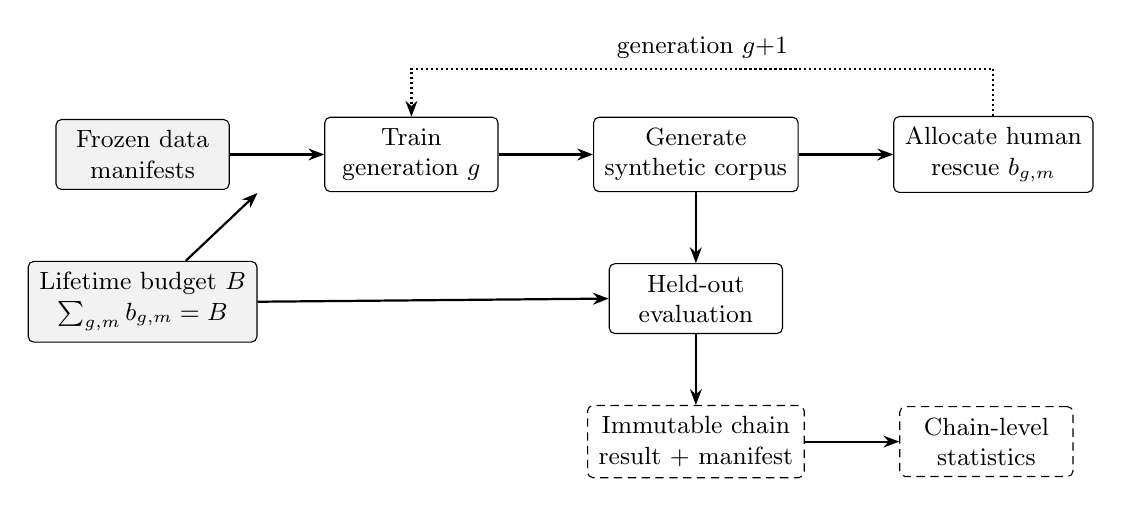
\begin{tikzpicture}[
  node distance=9mm and 12mm,
  every node/.style={font=\small},
  stage/.style={
    draw, rounded corners=2pt, align=center,
    minimum height=8mm, minimum width=22mm, inner sep=4pt
  },
  frozen/.style={stage, fill=black!5},
  artifact/.style={stage, densely dashed},
  flow/.style={-{Stealth[length=2mm]}, thick},
  feedback/.style={-{Stealth[length=2mm]}, thick, densely dotted},
]

  \node[frozen] (manifests) {Frozen data\\manifests};
  \node[stage, right=of manifests] (train) {Train\\generation $g$};
  \node[stage, right=of train] (generate) {Generate\\synthetic corpus};
  \node[stage, right=of generate] (allocate) {Allocate human\\rescue $b_{g,m}$};

  \node[frozen, below=of manifests] (budget) {Lifetime budget $B$\\$\sum_{g,m} b_{g,m} = B$};
  \node[stage, below=of generate] (evaluate) {Held-out\\evaluation};
  \node[artifact, below=of evaluate] (chain) {Immutable chain\\result + manifest};
  \node[artifact, right=of chain] (analysis) {Chain-level\\statistics};

  \draw[flow] (manifests) -- (train);
  \draw[flow] (train) -- (generate);
  \draw[flow] (generate) -- (allocate);

  % The recursion: this generation's allocation feeds the next generation's training.
  \draw[feedback] (allocate.north) -- ++(0,6mm) -| node[pos=0.25, above] {generation $g{+}1$} (train.north);

  \draw[flow] (budget) -- (allocate.south -| budget.east) ;
  \draw[flow] (budget.east) -- (evaluate.west);
  \draw[flow] (generate.south) -- (evaluate.north);
  \draw[flow] (evaluate) -- (chain);
  \draw[flow] (chain) -- (analysis);

\end{tikzpicture}

\caption{\textbf{The budgeted allocation problem.} A chain repeats
train\,$\rightarrow$\,generate\,$\rightarrow$\,allocate\,$\rightarrow$\,evaluate for a
frozen horizon; the dotted edge is the recursion, where generation $g$'s allocation enters
generation $g{+}1$'s training mixture. Shaded boxes are frozen before any run; dashed boxes
are immutable artifacts. \textbf{The lifetime budget $B$ couples every allocation
decision:} spending human tokens early leaves fewer for later generations, and spending
them on one monitored mode leaves fewer for the others. That coupling is what makes
\emph{when} and \emph{where} a single joint decision rather than two independent ones.}
\label{fig:pipeline}
\end{figure}

\paragraph{Contributions.}
\textbf{(i)} We formalise allocation of a fixed lifetime human-token stock as a joint
decision over recursive time and monitored modes, under exact matching of \emph{both}
lifetime human tokens and total optimizer tokens (Section~\ref{sec:problem}).
\textbf{(ii)} We decompose it into fresh-random, schedule-only, selection-only and joint
treatment families that isolate each axis (Section~\ref{sec:problem}).
\textbf{(iii)} We execute the comparison on \PilotChains{} chains and report a preregistered
null with an interval inside the equivalence region, together with three admissible
secondary contrasts that say where the effect actually lives (Section~\ref{sec:results},
Table~\ref{tab:results}).
\textbf{(iv)} We report what the design cannot support --- three unimplemented comparators
and an unarchived allocation trace --- rather than leaving the gaps to inference
(Section~\ref{sec:discussion}).

\section{Problem and policies}
\label{sec:problem}

\paragraph{Budgeted recursion.}
Over generations $g=0,\ldots,G-1$, each model trains on the previous generation's decoded
corpus plus human-origin examples bought by a policy, and optimization restarts from the
same pretrained base each generation so that what changes is the training distribution
rather than accumulated weights. Writing $b_{g,m}$ for human-origin tokens from monitored
mode $m$ consumed by the optimizer at generation $g$, every policy satisfies
$\sum_{g}\sum_{m} b_{g,m}=B$. Tokens are counted per optimizer presentation, so replaying
an example three times costs three times.

\paragraph{Matching both axes.}
Total optimizer tokens are held fixed as well. Rescued human examples \emph{displace}
synthetic records rather than being appended, so each generation's training volume is
constant regardless of what a policy buys. This matters more than it sounds: under additive
assembly the no-rescue control trains on strictly less data than every spending arm, and
``spending helps'' cannot then be separated from ``more data helps''. Displacement removes
that confound by construction.

\paragraph{Policy-visible state.}
Allocation may use only information available before the intervention: the generation index,
remaining budget, eligible candidates, the previous generation's monitoring statistics, and
the policy's own history. Final-test data never influences prompting, selection, thresholds,
stopping or hyperparameters.

\paragraph{Treatment families.}
\emph{Fresh-random} follows a frozen schedule and samples candidates without mode targeting.
\emph{Schedule-only} varies when to spend but distributes each generation's spend by a frozen
neutral mode rule. \emph{Selection-only} follows a fixed schedule but ranks candidates by the
lagged under-coverage of their mode. \emph{Joint} chooses both. A \emph{no-rescue} control
spends nothing. Appendix~\ref{sec:method} gives the allocation rules and frozen parameters.

\paragraph{Outcome.}
Let $L_g^{\pi}$ be held-out human NLL at generation $g$. Regret is measured against the
chain's \emph{own} generation-0 value, $r_g^{\pi}=L_g^{\pi}-L_0^{\pi}$, and the chain-level
outcome is the trapezoid area $A^{\pi}=\sum_{g=1}^{G-1}\tfrac12(r_{g-1}^{\pi}+r_g^{\pi})$.
The reference is within-chain, so a paired contrast inherits no variance from a shared
baseline. A frozen tail-retention measure on a disjoint partition is the confirmatory
outcome. One complete seeded chain is one experimental unit; generations within a chain are
repeated observations and are not independent samples.

\section{Experimental design}
\label{sec:experiments}

GPT-2 on WikiText-103, horizon $G=\PilotHorizon{}$, the frozen seed set
$\{101,202,303,404,505\}$, and a lifetime budget of \PilotCeiling{} optimizer-consumed human
tokens per spending arm. Five policies $\times$ \PilotSeeds{} seeds gives \PilotChains{}
chains. The primary estimand is the paired chain-level difference between joint and the
strongest eligible non-joint baseline, where ``strongest'' is fixed by a preregistered rule
and may not be chosen after seeing primary outcomes. The practical-effect threshold is
\PilotThresholdPct\% relative, frozen before outcomes were opened. Appendix~\ref{app:config}
gives the executed configuration, and Appendix~\ref{app:separation} the partition regime.

\section{Results}
\label{sec:results}

\paragraph{Both fairness axes hold.}
Realised lifetime human spend across the spending arms ranges from \PilotMatchedLow{} to
\PilotMatchedHigh{} tokens against a \PilotCeiling{} ceiling, a spread of
\PilotHumanSpreadPct\% against \PilotSpreadPermittedPct\% permitted. Realised total optimizer
tokens are \emph{identical} across all five arms, a spread of \PilotTotalSpreadExactPct\%.
All \PilotChains{} chains completed and none certifies invalid. The comparison is therefore
admissible, and what follows is a result rather than a precondition failure.

\begin{table}[t]
\centering
\caption{\textbf{Per-arm results; selection-only and joint are indistinguishable.} Every arm
is matched on both budget axes, so all rows are mutually comparable. AUC regret is the area
under the generation-wise held-out human NLL-regret curve against each chain's own
generation-0 value (lower is better); SD is between-chain standard deviation over
\PilotSeeds{} chains; tail retention is the confirmatory outcome at the final generation
(higher is better). Bold marks the best value in a column, and both arms are bolded where
they tie at displayed precision.}
\label{tab:results}
{\small% AUTO-GENERATED by scripts/generate_pilot_outputs.py. DO NOT EDIT VALUES BY HAND.
% Derived from chain_result.json artifacts of primary_pilot_v2_2026-08-20.
% Both budget axes hold, so the preregistered contrast is reported below the
% table. Strongest eligible non-joint baseline: selection_only.
\begin{tabular}{lrrrrr}
\toprule
Policy & Chains & Human tokens & AUC regret & SD & Tail retention \\
\midrule
No rescue (control) & 5 & 0 & 2.6431 & 0.0140 & 0.8676 \\
Fresh random & 5 & 749,869 & 2.5364 & 0.0080 & 0.8769 \\
Schedule-only & 5 & 749,878 & 2.5261 & 0.0194 & 0.8846 \\
Selection-only & 5 & 749,827 & 2.2931 & 0.0250 & 0.9024 \\
Joint time-and-mode & 5 & 749,827 & 2.3034 & 0.0221 & 0.9024 \\
\bottomrule
\end{tabular}

% Primary contrast, joint minus selection_only (paired by seed, 95\% t interval):
%   +0.01026 [-0.00916, +0.02968], +0.45\% relative.
%   Practical-equivalence region is +/-0.05073 (2\% of the fresh-random mean, the denominator U-006 was settled against).
%   Interval lies entirely inside that region: yes.
% Budget axes: human spread 0.0381\%, total spread 0.0000\%, permitted 0.2000\%.
}
\end{table}

\paragraph{The primary contrast is a null.}
The strongest eligible non-joint baseline is \PilotPrimaryBaseline{}. Across \PilotChains{}
chains at matched budgets we did not detect a difference between joint allocation and that
baseline: paired mean \PilotPrimaryMean{}, $95\%$ Student $t$ interval on four degrees of
freedom $[\PilotPrimaryLow, \PilotPrimaryHigh]$, or \PilotPrimaryPct\% relative. The frozen
practical-equivalence region is $\pm\PilotThresholdUnits{}$, and the interval lies entirely
inside it, reaching at most \PilotPrimaryReach{} from zero.

We report this as a null, not a trend. It is moreover the stronger form: the interval does
not merely include zero, it excludes every difference the preregistration calls practically
meaningful. The design is powered to detect effects at that threshold with roughly three
chains per arm and ran with \PilotSeeds{}, so this is equivalence rather than insufficient
power. Joint allocation is \emph{not} shown to be worse; the interval covers zero.

\paragraph{Where the effect actually is.}
Because every arm is matched on both axes, the secondary contrasts are admissible on the
same footing as the primary one.

\begin{itemize}\itemsep2pt
\item \textbf{Spending at all helps.} Fresh random against the no-rescue control improves the
      outcome by \PilotRandNonePct\%, CI $[\PilotRandNoneLow, \PilotRandNoneHigh]$, clearing
      the practical threshold. Under displacement this arm trains on exactly as much data as
      the control, so the gain is attributable to the data's \emph{origin}, not its quantity.
\item \textbf{Which examples you buy matters more.} Selection-only against fresh random
      improves it by \PilotSelRandPct\%, CI $[\PilotSelRandLow, \PilotSelRandHigh]$, at
      identical total volume.
\item \textbf{When you spend does not.} Schedule-only against fresh random gives
      \PilotSchedRandPct\%, CI $[\PilotSchedRandLow, \PilotSchedRandHigh]$, an interval
      containing zero and lying inside the equivalence region.
\end{itemize}

The primary null follows from these: selection accounts for most of the achievable
improvement, scheduling for none detectable on the primary outcome, and the joint policy
that combines them lands where selection alone lands.

\paragraph{The confirmatory outcome agrees, with one exception that we report.}
On the primary contrast tail retention agrees and more tightly: \PilotTailPrimaryMean{}, CI
$[\PilotTailPrimaryLow,\allowbreak\ \PilotTailPrimaryHigh]$. On the \emph{timing} contrast it
disagrees: \PilotTailSchedRandMean{}, CI
$[\PilotTailSchedRandLow,\allowbreak\ \PilotTailSchedRandHigh]$, an interval excluding zero
at \PilotTailSchedRandPct\% of the fresh-random level. We do not select the more favourable
metric. The primary conclusion follows the primary outcome, and the honest summary is that
timing shows no detectable effect on chain-level regret and a small, statistically
distinguishable, practically minor effect on tail retention.

\begin{figure}[t]
\centering
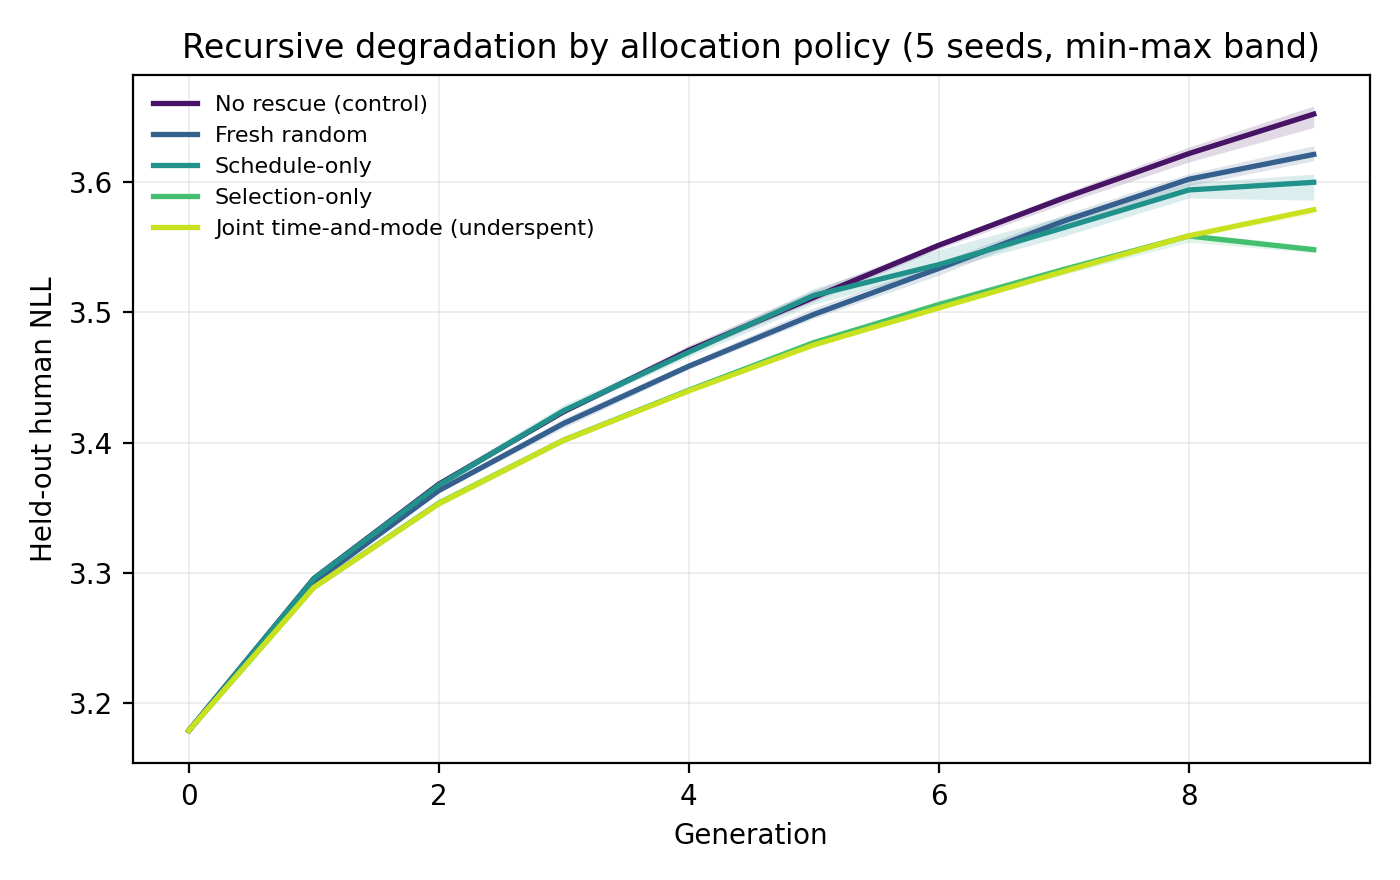
\includegraphics[width=0.78\linewidth]{pilot_nll_by_generation}
\caption{\textbf{Held-out human NLL by generation; the two targeted policies coincide.}
Mean over the frozen seed set with a min--max band. Every policy that spends its budget ends
below the no-rescue control, and the selection-only and joint trajectories lie on top of one
another for the whole horizon --- the primary null shown rather than stated. All five arms
consumed identical total optimizer tokens, so the separation between trajectories is not
attributable to differences in training volume.}
\label{fig:nll}
\end{figure}

\paragraph{Variance.}
Between-chain coefficients of variation run \PilotCVLow\%--\PilotCVHigh\% against the
\PilotThresholdPct\% threshold, reproducing on an independent grid the estimate that sizes
this design. Chain count is not the binding constraint here; baseline coverage is.

\section{Discussion and limitations}
\label{sec:discussion}

The question this work poses decomposes at the operating point measured, and the primary
outcome carries signal on one half of it: which under-covered modes a fixed human budget
targets changes chain-level regret, and when within the chain it is spent does not. Adding
scheduling to targeting is equivalent to targeting alone.

Four limits bound that statement, and each is a reason not to read it more widely.
\textbf{One operating point:} GPT-2, WikiText-103, horizon \PilotHorizon{}, one budget, one
corpus-assembly rule. \textbf{Missing comparators:} three of the seven predeclared
comparators were never implemented --- accumulation or fixed-fraction mixing, detector-based
selection, and oracle mode information as a non-deployable upper bound. The absent oracle is
the consequential one: an equivalence between two policies carries no information about how
much of the achievable gain either captures, and a reader should not infer that
selection-only sits near a ceiling. \textbf{An unarchived trace:} the retained artifacts
record how much each policy spent but not \emph{when} or on which modes, so whether the joint
policy reached its total by a different route than selection-only cannot be determined; an
equivalence between two policies that allocated differently means something different from
one between two policies that converged. \textbf{An unreviewed threshold:} the
practical-equivalence bound has been checked against measured anchors and never externally
reviewed, and an equivalence rests on it more directly than a positive finding would.
Under the alternative denominator the region is $\pm\PilotThresholdUnitsAlt{}$ and the
verdict is unchanged.

What would move this forward is not more chains. It is the comparators that were not built
--- an oracle mode-information upper bound above all --- and operating points beyond the
single one measured here.

\bibliographystyle{plain}
\bibliography{references}

% The appendix reuses the full paper's sections verbatim rather than restating them,
% so the workshop version cannot drift from paper/main.tex. 10_appendix.tex issues its
% own \appendix, which is why none is issued here.
\appendix

\section{Experimental Apparatus}
\label{app:apparatus}

Figure~\ref{fig:pipeline} shows the recursive procedure. One \emph{chain} is one
independently seeded traversal of the loop for the full horizon $G$. Chains, not
generations, are the experimental units: generations within a chain are repeated
observations of the same trajectory and are not independent samples.

\begin{figure}[h]
\centering
% Recursive train/generate/allocate/evaluate pipeline.
% Result-independent: this figure describes the experimental apparatus, not any
% outcome, so it is safe to include before results exist.
% Requires \usepackage{tikz} and \usetikzlibrary{arrows.meta,positioning} in main.tex.
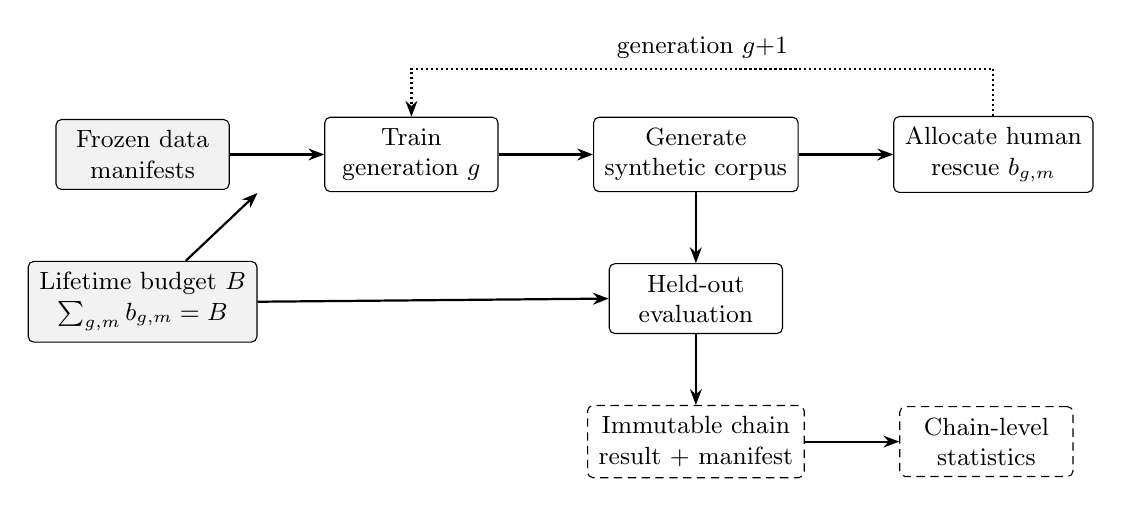
\begin{tikzpicture}[
  node distance=9mm and 12mm,
  every node/.style={font=\small},
  stage/.style={
    draw, rounded corners=2pt, align=center,
    minimum height=8mm, minimum width=22mm, inner sep=4pt
  },
  frozen/.style={stage, fill=black!5},
  artifact/.style={stage, densely dashed},
  flow/.style={-{Stealth[length=2mm]}, thick},
  feedback/.style={-{Stealth[length=2mm]}, thick, densely dotted},
]

  \node[frozen] (manifests) {Frozen data\\manifests};
  \node[stage, right=of manifests] (train) {Train\\generation $g$};
  \node[stage, right=of train] (generate) {Generate\\synthetic corpus};
  \node[stage, right=of generate] (allocate) {Allocate human\\rescue $b_{g,m}$};

  \node[frozen, below=of manifests] (budget) {Lifetime budget $B$\\$\sum_{g,m} b_{g,m} = B$};
  \node[stage, below=of generate] (evaluate) {Held-out\\evaluation};
  \node[artifact, below=of evaluate] (chain) {Immutable chain\\result + manifest};
  \node[artifact, right=of chain] (analysis) {Chain-level\\statistics};

  \draw[flow] (manifests) -- (train);
  \draw[flow] (train) -- (generate);
  \draw[flow] (generate) -- (allocate);

  % The recursion: this generation's allocation feeds the next generation's training.
  \draw[feedback] (allocate.north) -- ++(0,6mm) -| node[pos=0.25, above] {generation $g{+}1$} (train.north);

  \draw[flow] (budget) -- (allocate.south -| budget.east) ;
  \draw[flow] (budget.east) -- (evaluate.west);
  \draw[flow] (generate.south) -- (evaluate.north);
  \draw[flow] (evaluate) -- (chain);
  \draw[flow] (chain) -- (analysis);

\end{tikzpicture}

\caption{Recursive train--generate--allocate--evaluate pipeline. Shaded boxes are
frozen before any run. Dashed boxes are immutable artifacts. The dotted edge is
the recursion: generation $g$'s allocation enters generation $g{+}1$'s training
mixture. The lifetime budget constrains every allocation jointly, so spending
early reduces what remains for later generations.}
\label{fig:pipeline}
\end{figure}

\section{Data Appendix}
\label{app:data}

\textbf{RESULT\_PENDING.} The primary domain is not yet frozen
(\texttt{DECISIONS.md} U-002). This appendix records what will be reported once it
is, and is structured so that filling it requires no reorganisation.

\begin{itemize}
  \item Dataset identifier, revision hash, and licence, with the licence audit
    that selected it over the audited alternatives.
  \item Preprocessing: tokenizer identity and revision, normalisation, and the
    exact filter chain, each with a content hash.
  \item Partition statistics for all five partitions --- base training, rescue
    candidates, prompts, validation, and final test --- reporting example counts,
    token counts, and per-partition manifest hashes.
  \item The frozen mode definition, the number of modes $M$, and the criterion
    separating tail modes from common modes.
  \item Overlap report: exact and near-duplicate checks across every partition
    pair, with the near-duplicate threshold declared before it was applied.
\end{itemize}

Final test data influences no prompt, selection decision, threshold, stopping
rule, or hyperparameter. This constraint is enforced by the disjointness tests
rather than asserted.

\section{Evaluation Appendix}
\label{app:evaluation}

\textbf{RESULT\_PENDING.} The primary tail-retention definition is not yet frozen
(U-004). Two candidates are implemented and audited for determinism,
independence from the policy's selection signal, sensitivity to tail degradation,
discriminant validity against non-tail modes, and split-half reliability.

Held-out human negative log-likelihood is computed from target-token log
probabilities on the frozen test partition. Regret is aggregated across the
horizon as the area under the generation-wise curve.

Both tail candidates are computed without reference to the policy's
under-coverage score, so no policy can be rewarded for agreeing with its own
selection signal. This is a structural property of the interfaces, not a
convention.

\section{Statistics Appendix}
\label{app:statistics}

\textbf{RESULT\_PENDING.} Uncertainty is computed across independent chains.
Multiple generations within one chain are repeated observations and do not
increase the effective sample size.

The primary contrast is the joint policy against the strongest eligible non-joint
baseline, paired by chain seed. Paired differences are summarised by their mean
with a bootstrap interval resampled over complete chains. The smallest
scientifically meaningful effect is frozen before outcomes are opened (U-006),
and the interpretation that follows is selected mechanically from precommitted
templates covering favourable, null, harmful, and uncertain outcomes.

\section{Reproducibility Appendix}
\label{app:reproducibility}

Every value reported in this paper is generated by a script and traced to an
immutable artifact. No number is entered by hand.

\begin{itemize}
  \item \textbf{Positive control.} Upstream repository and exact commit are
    pinned before execution, together with the resolved framework versions and
    tokenizer revision actually used. Deviations from the upstream configuration
    are declared before running, never after observing a result.
  \item \textbf{Run artifacts.} Each chain emits a run manifest and a chain
    result validated against versioned JSON schemas. A three-state validator
    classifies each run as valid, valid with limitation, or invalid; blocking
    failures include budget-equality violations, identity mismatches, and
    impossible token accounting.
  \item \textbf{Budget matching.} Every policy in a comparison consumes identical
    lifetime human-origin optimizer tokens and identical total optimizer tokens.
    Equality is checked before launch from configuration and again after the run
    from emitted artifacts.
  \item \textbf{Token accounting.} Counts derive from tokenized batches actually
    consumed by the optimizer. Repeated presentation of an example costs its
    tokens once per presentation; gradient accumulation counts every micro-batch;
    resume neither double-counts nor drops the batch spanning a checkpoint.
  \item \textbf{Determinism.} Seeds propagate through sampling, generation,
    initialisation, dropout, and evaluation. Checkpoints carry content digests so
    silent corruption cannot survive a resume.
  \item \textbf{Generated outputs.} Tables and figures are emitted by scripts and
    recorded with SHA-256 digests in an artifact manifest, so a reader can verify
    that a figure is the one the pipeline produced.
\end{itemize}

\section{Limitations of Scope}
\label{app:scope}

\textbf{RESULT\_PENDING.} The planned study covers one licensed domain, one
124M--160M screening model, and one horizon. It cannot establish behaviour at
larger scales, in other domains, or for other model families. Any claim beyond
the tested configuration is future work and is marked as such.

\section{Method}
\label{sec:method}

\subsection{Setting}

A model is trained recursively: each generation $g \in \{0,\dots,H-1\}$ trains on data drawn
from the previous generation's outputs, optionally supplemented with human-origin examples.
The quantity under allocation is a \emph{fixed lifetime budget} $B$ of human-origin
optimizer tokens. A policy decides, at each generation, how much of the remaining budget to
spend and which candidates to spend it on. Every policy in a budget-matched comparison
consumes exactly the same lifetime human-origin token count and the same total
optimizer-token count.

\subsection{Policy-visible state}

At generation $g$ a policy observes only the remaining human-token budget, the number of
generations remaining, and a monitored per-mode under-coverage score computed from a lagged
reference. It does not observe held-out test data, another policy's outputs, or any primary
treatment outcome. A partially missing mode receives score zero; if every mode is missing,
selection falls back to a seeded random candidate order.

\subsection{Treatment families}

Four budget-matched families are compared. Let $r$ denote remaining human tokens, $F$ the
number of future generations, $s_{\text{base}}$ the base per-generation spend, and
$s_{\max}$ the per-generation cap.

\paragraph{Fresh random rescue.} Spend $\min(s_{\text{base}}, r)$ each generation; shuffle
candidates under the supplied seed and select without exceeding budget.

\paragraph{Schedule-only.} Spend $s_g$ from a frozen schedule that withholds tokens through
the early generations and spends at the cap thereafter; select in seeded random order.
Timing varies; mode targeting does not.

\paragraph{Selection-only.} Spend $\min(s_{\text{base}}, r)$ each generation; score
candidates by lagged mode under-coverage, sort descending, break ties by ascending example
identifier. Mode targeting varies; the spending schedule does not.

\paragraph{Joint time-and-mode.} Let $u$ be the maximum finite monitored mode score, and let
$\tau_{\text{low}} < \tau_{\text{high}}$ be the frozen urgency thresholds. The desired spend
is
\[
d(u) = \begin{cases}
0 & u < \tau_{\text{low}}\\
s_{\text{base}} & \tau_{\text{low}} \le u < \tau_{\text{high}}\\
s_{\max} & u \ge \tau_{\text{high}}
\end{cases}
\]
and the realised spend applies a feasibility clamp,
\[
b = \mathrm{clamp}\bigl(d(u),\; \max(0,\, r - s_{\max}F),\; \min(s_{\max},\, r)\bigr).
\]
The lower bound reserves enough budget that every remaining generation can still be served
at the cap; the upper bound enforces the per-generation cap and the remaining budget.
Candidates are then sorted by descending score, ties broken by ascending example identifier.

\subsection{Why the joint policy is not two tuned baselines composed}

This is the load-bearing design question, and it is settled by an eligibility constraint
rather than by an empirical margin.

Schedule-only may alter \emph{when} tokens are spent but may not choose \emph{which} modes
receive them. Selection-only may choose modes but spends on a fixed schedule. Composing a
tuned schedule-only policy with a tuned selection-only policy yields a fixed spending
profile paired with mode-aware selection: the schedule is still chosen in advance and cannot
respond to what monitoring reports at run time.

The joint policy is the only eligible family whose spend at generation $g$ is a function of
the monitored state at generation $g$. The urgency thresholds make spending reactive --- a
generation whose worst monitored mode is well covered spends nothing, and one whose worst
mode is badly covered spends the cap. Under a fixed lifetime budget this is a reallocation,
not an increase: tokens withheld early remain available later, and the feasibility clamp
guarantees the reserve never falls below what future generations require.

Whether that reactivity helps is an empirical question this paper does not answer.

\subsection{Frozen parameters}

\begin{table}[h]
\centering
\caption{Frozen policy parameters, generated from \texttt{configs/policy/joint.json}.}
% AUTO-GENERATED by scripts/generate_method_tables.py. DO NOT EDIT VALUES BY HAND.
\begin{tabular}{lr}
Frozen parameter & Value \\
\hline
Horizon & 10 \\
Lifetime human tokens & 100 \\
Base generation spend & 10 \\
Maximum generation spend & 20 \\
Token granularity & 10 \\
Monitoring lag (generations) & 1 \\
\hline
Desired spend, $u < 0.25$ & 0 \\
Desired spend, $0.25 \le u < 0.50$ & 10 \\
Desired spend, $u \ge 0.50$ & 20 \\
\end{tabular}

\end{table}

These were fixed in the Week~2 method freeze using interfaces, fixtures, and synthetic
results. No primary treatment outcome influenced any score, schedule, seed, threshold,
exclusion rule, or interpretation.

\subsection{Separation of the treatment families}

An earlier internal finding recorded the joint and selection-only families as
observationally identical, and random as identical to schedule-only. That finding was
subsequently traced to a reverted implementation rather than to the method: with the frozen
rule restored, all four families produce distinct trajectories under the fixture simulator,
and random separates from schedule-only. This evidence is structural and fixture-based. It
establishes that the decomposition is well posed; it is not evidence of any performance
difference on real data.

\section{Related Work}
Ronit will complete a hostile closest-work review covering recursive degradation, accumulation and replacement, fresh human mixing, importance resampling, semantic and surprise sampling, data scheduling, and monitoring bias. The exact novelty statement remains provisional until that review and an external review are complete. See the repository evidence registry rather than treating this placeholder as a literature claim.


\end{document}
